\section{Properties of Pure Substances}\label{sec:Properties_Pure_Substances}
Many of the substances that we study in \nameref{def:Thermodynamics} are what we call \nameref{def:Pure_Substance}s.

\begin{definition}[Pure Substance]\label{def:Pure_Substance}
  A \emph{pure substance} is one whose chemical composition is fixed throughout.
  Properties of these substances are completely known, and these properties are completely uniform throughout the substance.
\end{definition}

In general, the pressure of a substance is an exponential function that is dependent on the temperature of the water.
In addition, the pressure of the substance depends on its altitude.
As you increase in altitude, this means that the temperature required to boil the substance at decreases.
All of these are visualized in \Cref{fig:Temp_Pressure_Liquid_Vapor_Curve}.

\begin{figure}[h!tbp]
  \centering
  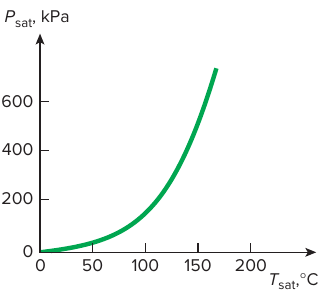
\includegraphics[scale=0.75]{./Temperature_Pressure_Liquid_Vapor_Curve.png}
  \caption{Temperature-Pressure ($\Temp$-$\Pressure$) Liquid-Vapor Curve}
  \label{fig:Temp_Pressure_Liquid_Vapor_Curve}
\end{figure}

\subsection{Phase Changes}\label{subsec:Phase_Changes}
Phase changes in materials are unique, because they maintain a constant temperature \textbf{until} all the material undergoes the phase change, however, the volume increases \textbf{drastically}.

\begin{definition}[Phase Change]\label{def:Phase_Change}
  A \emph{phase change} in a substance is when it changes from one state of matter to another.
  This means a substance goes from solid to liquid, liquid to gas, gas to solid, solid to gas, etc.
  Each of these ``directions'' has a name:
  \begin{description}[noitemsep]
  \item[Solid to Liquid:] Melting/Fusion
  \item[Liquid to Solid:] Solidification/Crystallization
  \item[Liquid to Gas:] Evaporation/Vaporization
  \item[Gas to Liquid:] Condensation
  \item[Solid to Gas:] Sublimation
  \item[Gas to Solid:] Desposition
  \end{description}
\end{definition}


%%% Local Variables:
%%% mode: latex
%%% TeX-master: "../MMAE_320-Thermo-Reference_Sheet"
%%% End:
